\section{レポート課題1}
\subsection{課題1}
ロジスティク写像の時系列変化を計算するプログラムを作成し、$r = 1.50, r = 2.60,r = 3.20, r = 3.50,$ \par
$r = 3.86, r = 3.90 のとき、x0 = 0.7$として個体数変動の時系列グラフを表示せよ。\par

\subsection{課題2}
ロジスティク写像のリターンマップを描くためのプログラムを作成し、$r = 1.50, r = 2.60, r = 3.20,$ \par
$r = 3.50, r = 3.86, r = 3.90 のとき、x0 = 0.7$として個体数変動のリターンマッ
プを表示せよ。グラフには、$x_{n+1} = r(1 −x_n)x_n とx_{n+1} = x_n$ のグラフも表示すること。\par
画像:
\begin{figure}[htbp]
  \begin{tabular}{cc}
    \begin{minipage}[t]{0.45\hsize}
      \centering
      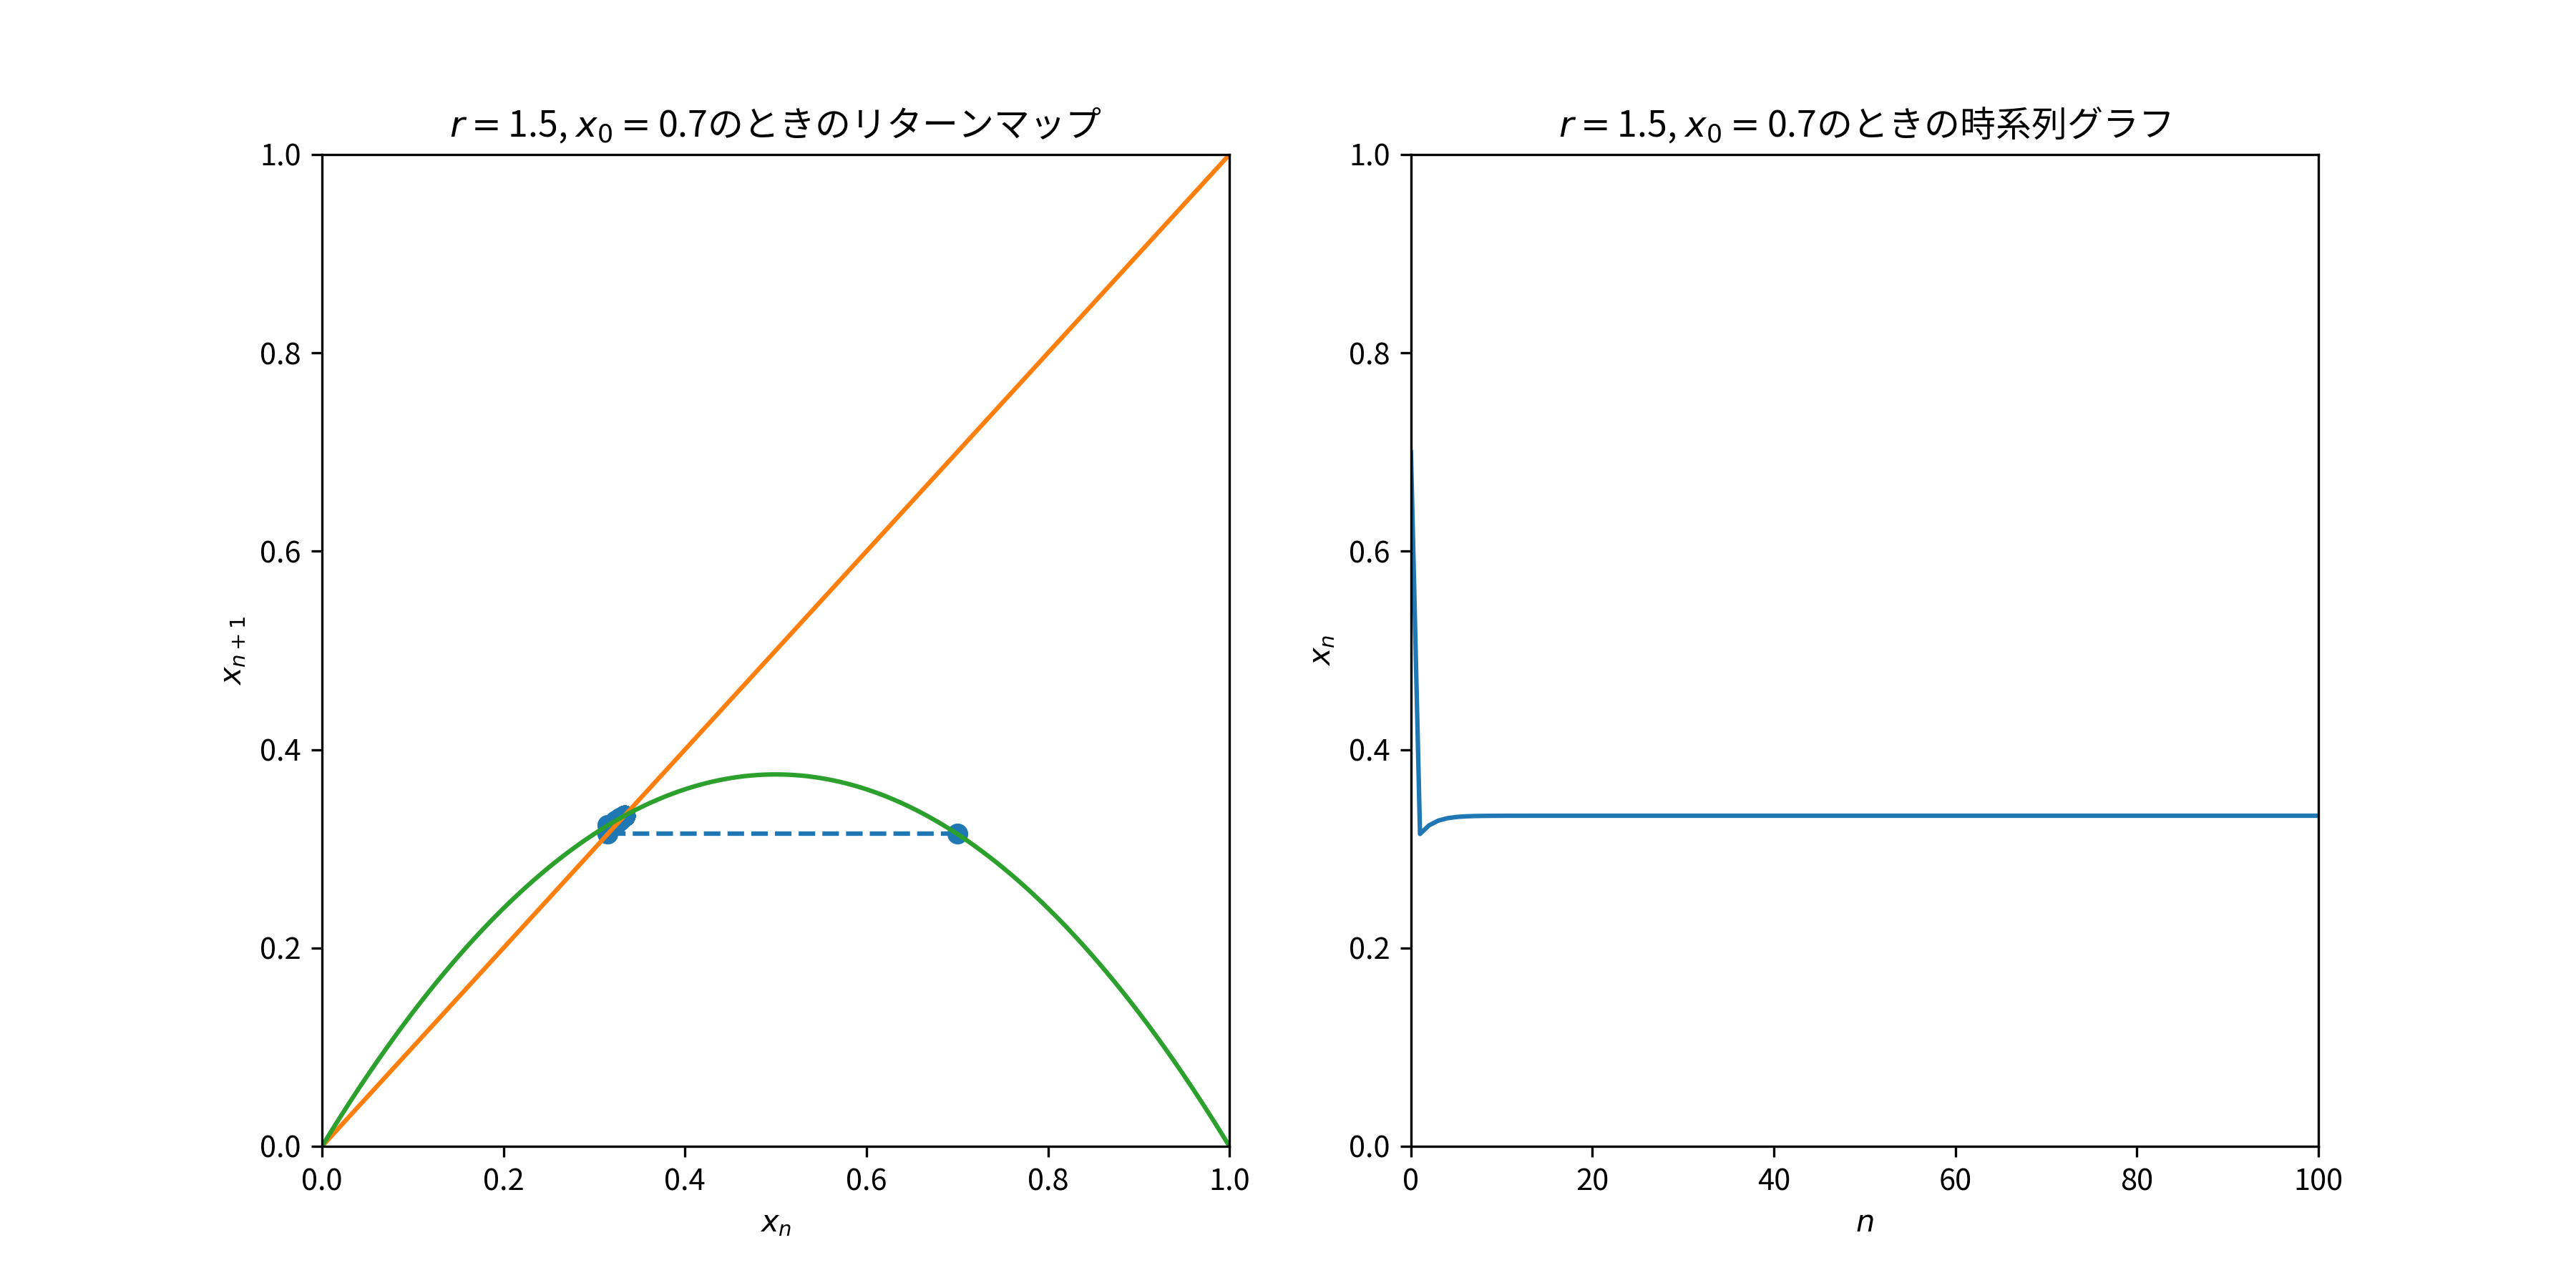
\includegraphics[keepaspectratio, scale=0.25]{images/ctest2_1.png}
    \end{minipage}

    \begin{minipage}[t]{0.45\hsize}
      \centering
      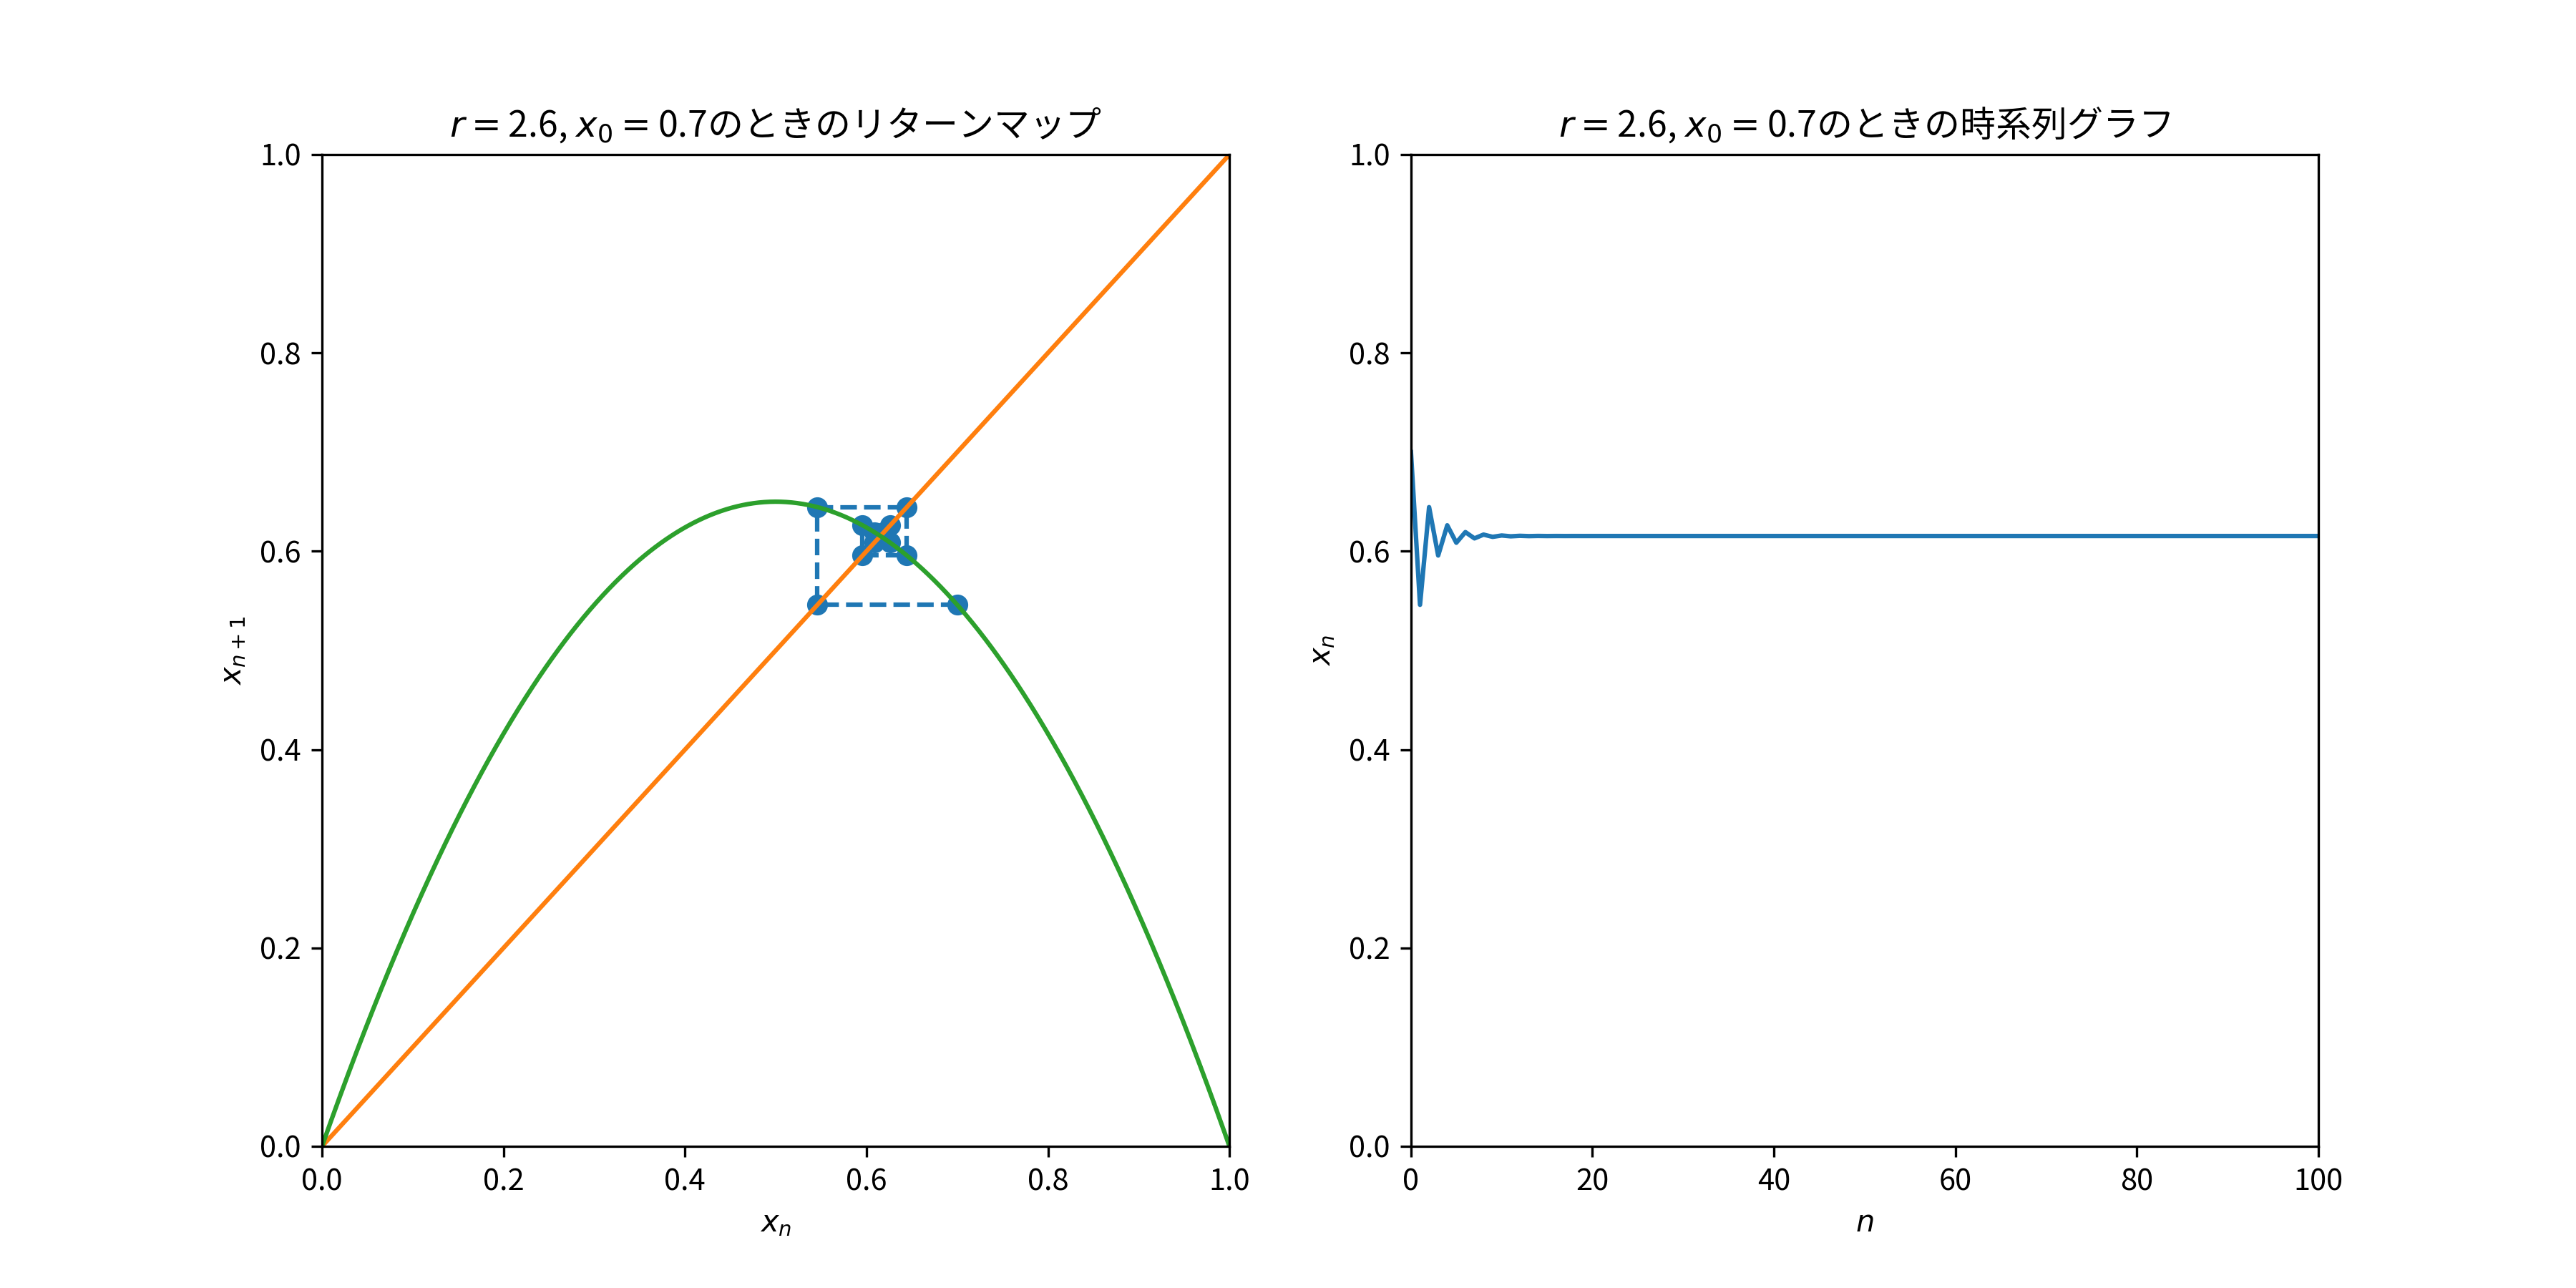
\includegraphics[keepaspectratio, scale=0.25]{images/ctest2_2.png}
    \end{minipage}
  \end{tabular}
\end{figure}

解説:\par
この図は左にリターンマップ、右に時系列グラフをレポートの$r$に合わせてプロットしたものである。
\begin{itemize}
  \item 時系列グラフは、ロジスティック回帰の各 $0 \leq n \leq 100$ のときの $x_n$ を計算しプロットしている。$x$ 軸は $n$ を、$y$ 軸には $x_n$ をプロットしている。\par
    この図から$r$の値によって挙動が変わっているのが読み取れる。$r = 1.50, 2.60$ のときには $n$ を増加させていくと $x_n$ が収束していく。また、$r = 3.20, 3.50$ のときには $n$ を増加させていくと $x_n$ に周期性が見られるようになる。さらに、$r = 3.86, 3.90$ のときには $n$ を増加させていくと $x_n$ に周期性は現れることなく値が収束することもない。\par
    この考察から、ロジスティック回帰は $r$ の値を変化させていくことでカオスの条件を満たす場合と満たさない場合がある。\par
    
  \item リターンマップは、
\end{itemize}
